\linespread{1.3}
\section{Задание 4. Приложение Рядов. Шпинева Ульяна. Вариант 6}
\subsection{Задание 1}
Вычислить приближенно значение функции $ \frac{1}{\sqrt[3]{e^2}} $ с точностью 0,0001\\
\begin{flushright}
\begin{minipage}{15cm}
	\text{Возьмем табличное разложение}\\
	$e^x =  \sum_{k=0}^{\infty} \frac{x^n}{n!}$\\
	$e^{-\frac{2}{3}} =  \sum_{k=0}^{\infty} \frac{(-\frac{2}{3})^n}{n!}$\\
	\text{$n = 0:$}
	$$\frac{(-\frac{2}{3})^0}{0!} = 1$$\\
	\text{$n = 1:$}
	$$  \frac{(-\frac{2}{3})^1}{1!} \approx -0,66667 $$\\
	\text{$n = 2:$}
	$$\frac{(-\frac{2}{3})^2}{2!} \approx 0,22222$$\\
	\text{$n = 3:$}
	$$\frac{(-\frac{2}{3})^3}{3!} \approx -0,04938$$\\
	\text{$n = 4:$}
	$$\frac{(-\frac{2}{3})^4}{4!} \approx 0,00823$$\\
	\text{$n = 5:$}
	$$\frac{(-\frac{2}{3})^5}{5!} \approx -0,00109$$\\
	\text{$n = 6:$}
	$$\frac{(-\frac{2}{3})^6}{6!} \approx 0,00012$$\\
	\text{$n = 7:$}
	$$\frac{(-\frac{2}{3})^7}{7!} \approx -0,00001$$\\
\end{minipage}\\
\end{flushright}
	\text{Дальнейшие члены не будут изменять точность}\\
	 $ \frac{1}{\sqrt[3]{e^2}} \approx 1 - 0,66667 + 0,22222 - 0,04938 + 0,00823 - 0,00109 + 0,00012 - 0,00001 = 0,51342 $\\

Проверка:
\begin{center}
	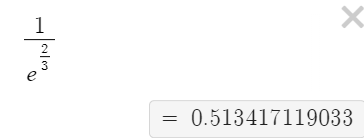
\includegraphics[width=.3\linewidth]{1_proof.png}\quad
\end{center}
\newpage
\subsection{Задание 2}
Разлагая подынтегральную функцию в степенной ряд вычислить приближенно интеграл с точностью 0,0001\\
\begin{equation*}
	\int_0^{\frac{1}{2}}ln(1 + x^4) dx
\end{equation*}
\begin{flalign*} 
	&\text{Возьмем табличное разложение}&&\\
	&\int_0^{\frac{1}{2}} ln(1 + x^4) dx = 
	\int_0^{\frac{1}{2}} \sum_{n=1}^\infty \frac{(-1)^{n-1} x^{4n}}{n} dx =
	\sum_{n=1}^\infty \int_0^{\frac{1}{2}} \frac{(-1)^{n-1} x^{4n}}{n} dx = 
	=\sum_{n=1}^\infty \frac{(-1)^{n-1}x^{4n+1}}{n(4n+1)} \bigg|_0^{\frac{1}{2}} =  &&\\
	&\sum_{n=1}^\infty \frac{(-1)^{n-1}}{n2^{4n+1}(4n+1)} &&\\
\end{flalign*}

Подсчитаем первые члены последовательности:
\begin{flalign*} 
	\text{$n = 1:$}& &&\\
	&\frac{1}{2^{5}\cdot 5} \approx 0,00625&&\\
	\text{$n = 2:$}& &&\\
	&\frac{-1}{2 \cdot 2^{9} \cdot 9} \approx -0,00011&&\\
	\text{$n = 3:$}& &&\\
	&\frac{1}{3 \cdot 2^{13} \cdot 13} \approx 0&&\\
	\text{Дальнейшие члены не будут изменять точность}& &&\\
	\int_0^{\frac{1}{2}}ln(1 + x^4) dx \approx 0,00625 &- 0,00011 = 0,00614
\end{flalign*}

Проверка:
\begin{center}
	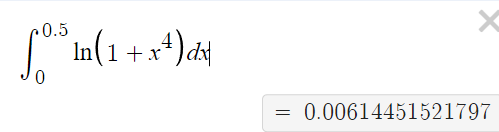
\includegraphics[width=.3\linewidth]{2_proof}\quad
\end{center}

\subsection{Задание 3}
Найти в виде степенного ряда решение дифференциального уравнения,
удовлетворяющего заданным начальным условиям. Ограничиться четырьмя
членами ряда.
\begin{flalign*}
	&y' = y^2 - 3x \\
	&y(1) = 2 \\
\end{flalign*}
\begin{flalign*}
	\text{Решение в виде ряда Тейлора: }& &&\\
	&y(x) = y(1) + y'(1)(x - 1) + \frac{y''(1)(x - 1)^2}{2!} + \frac{y'''(1)(x - 1)^3}{3!}&&\\
	1) \ &y' = y^2 - 3x &&\\
	&y'(1) = 2^2 - 3 = 1 &&\\
	2) \ &y'' = (y^2 - 3x)' = 2yy' - 3 &&\\
	&y''(1) = 2 \cdot 2 \cdot 1 - 3 = 1 &&\\
	3) \ &y''' = (2yy' - 3)' =  2y'y' + 2yy''&&\\
	&y'''(1) = 2 \cdot 1 \cdot 1 + 2 \cdot 2\cdot 1 = 6 &&\\
	\text{Подставим значения в ряд: }& &&\\
	&y(x) = y(1) + y'(1)(x - 1) + \frac{y''(1)(x - 1)^2}{2!} + \frac{y'''(1)(x - 1)^3}{3!} = &&\\
	&= 2 + (x - 1) + \frac{(x - 1)^2}{2} + (x - 1)^3 &&\\
\end{flalign*}
